\documentclass[10pt,letterpaper,compsoc,conference]{iiswc26}

%% INCLUDED PACKAGES: DO NOT REMOVE ANY OF THESE
\usepackage{cite}
\usepackage{amsmath,amssymb,amsfonts}
%\usepackage{algorithmic}
\usepackage{graphicx}
\usepackage[dvipsnames]{xcolor}
\usepackage[final]{microtype}
\usepackage[italic]{mathastext}
%\usepackage{libertine}   % requires texlive-fonts-extra
\usepackage[T1]{fontenc}
\usepackage{textcomp}
%\usepackage[varqu,varl]{zi4}  % requires texlive-fonts-extra
\usepackage[all]{nowidow}
%\usepackage[auth-lg,affil-it]{authblk}
\usepackage[keeplastbox]{flushend}
\usepackage{fancyhdr}
\usepackage{enumitem}
\usepackage{comment}

\newcommand{\BL}[1]{\textcolor{red}{[BL]#1}}
\newcommand{\SA}[1]{\textcolor{blue}{[SA]#1}}

\usepackage{tikz}
\newcommand{\circnum}[1]{%
\tikz[baseline=(char.base)]{
\node[
    shape=circle,
    fill=black,
    text=white,
    inner sep=1pt,
    font=\scriptsize
] (char) {#1};}}

%% ADD YOUR OTHER PACKAGES HERE
\usepackage{booktabs}
\usepackage{multirow}
\usepackage{array}
\usepackage{caption}
\captionsetup[table]{
  justification=raggedright,
  singlelinecheck=false,
  format=plain,
  labelfont={bf,sc},
  textfont=bf,            % ← makes the caption body bold too
  labelsep=quad           % ← adds a small horizontal gap between "TABLE 2:" and the title
}




\providecommand{\BibTeX}{\textsc{Bib}\TeX}
\graphicspath{{figs/}}
\newcommand{\figwidth}{\columnwidth}  % full column width (no overfull hbox)

% Placeholder marker for incomplete/pending data
\newcommand{\pending}[1]{\textcolor{red}{\textbf{[PENDING: #1]}}}

%% ADD YOUR OTHER PACKAGES ABOVE THIS LINE

%%%%%%%%%%% ---SETME-----%%%%%%%%%%%%%
\newcommand{\iiswcsubmissionnumber}{411}
%%%%%%%%%%%%%%%%%%%%%%%%%%%%%%%%%%%%

\fancypagestyle{firstpage}{
  \fancyhf{}
  \renewcommand{\headrulewidth}{0pt}
  \fancyhead[C]{\vspace{10pt}\normalsize{IISWC 2026 Submission
      \textbf{\#\iiswcsubmissionnumber} -- Confidential Draft -- Do
      NOT Distribute!!} \\\vspace{-25pt}}
  \fancyfoot[C]{\thepage}
}

\begin{document}


%% EDIT TITLE BELOW

\title{Dead on Arrival: Characterizing and Protecting Against Dead-Entry TLB Misses in GPU Microarchitectures}

%% DO NOT EDIT THE FOLLOWING

%\renewcommand\Authsep{\qquad}
%\renewcommand\Authand{\qquad}
%\renewcommand\Authands{\qquad}


%% EDIT AUTHOR LIST BELOW
%% DOUBLE-BLIND SUBMISSION: author block intentionally commented out

%\author{Author1 Name}
%\author{Author2 Name}
%\author{Author3 Name}
%\affil{Full Name of Awesome School}


%%% ALTERNATIVE FORMAT FOR MULTIPLE SCHOOLS:
%%%
% \author[1]{Author1 Name}
% \author[2]{Author2 Name}
% \author[2]{Author3 Name}
% \author[1]{Author4 Name}
% \affil[1]{Full Name of Awesome School}
% \affil[2]{Full Name of Awesomer School}


\maketitle
\thispagestyle{firstpage}
\pagestyle{plain}

%% EDIT YOUR PAPER'S CONTENTS BELOW

\begin{abstract}
GPU workloads with large memory footprints frequently suffer from redundant L2 TLB misses
in which a recently evicted translation is immediately re-walked at full page-walk cost.
We characterize these \emph{dead-entry misses} across 24 GPU workloads, finding they
account for up to 99\% of L2 TLB misses in the most TLB-sensitive applications, yet their
performance impact varies widely depending on memory access structure.
Workloads where warps share the same virtual page suffer from burst amplification, where
a single eviction stalls many warps simultaneously waiting for one translation to return.
In contrast, workloads where each warp accesses a distinct set of pages face a
capacity-overflow problem that no replacement policy can resolve, a distinction validated
by huge page experiments.
Building on this two-class taxonomy, we design \emph{DEPOT} (Dead-Entry PrOTection),
a 1\,KB Bloom filter mechanism that prevents recently evicted translations from being
displaced immediately upon reinstallation, delivering up to 72\% IPC improvement on
interference-driven workloads with zero overhead on others, and composing with the state-of-the-art TLB prefetching and compaction mechanism,
for 2 to 7\% additional gain.
\end{abstract}


\begin{IEEEkeywords}
GPU address translation, TLB, MSHR, memory hierarchy
\end{IEEEkeywords}
\section{Introduction}
\label{sec:introduction}

Address translation is a first-order performance concern in modern GPU workloads~\cite{power_x86}.
As applications move toward larger, irregular memory footprints such as sparse graph
traversal, scientific stencils, and machine learning inference over large embedding tables,
the GPU L2 TLB becomes a sustained bottleneck \cite{ganguly_interplay, shin_irregular}.
Prior work has approached this problem almost exclusively from an access-pattern perspective,
predicting which virtual pages will be needed next and prefetching their translations
before the demand miss occurs~\cite{latpc,valkyrie, mosaic, snake_prefetch}.
This framing implicitly treats each TLB miss as a cold event requiring a fresh page walk,
but many TLB misses are not cold at all. A \emph{dead-entry TLB miss} occurs when a virtual page whose translation is still valid
is evicted from the TLB and then re-accessed before the working set rotates again.
The page walk is not cold; it is redundant.
The entry was alive, was discarded by LRU replacement, and is now being reconstructed
at full page-walk cost.
Measuring this phenomenon across 24 GPU workloads reveals that dead-entry misses are
pervasive: in the most TLB-sensitive applications, over 99\% of all L2 TLB misses
carry an eviction-history signature.

\begin{figure}[t]
  \centering
  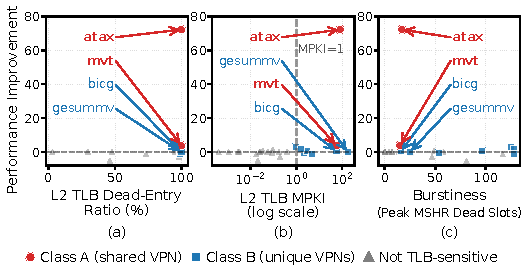
\includegraphics[width=\figwidth]{figs/fig01_teaser.pdf}
  \caption{Performance improvement (IPC) from eliminating dead-entry re-walks against three candidate predictors: (a)~DE ratio, (b)~MPKI, and (c)~MSHR burstiness, for all 24 workloads.}
  \label{fig:teaser}
\end{figure}

Yet the performance consequences of dead-entry misses are not uniform, and
Figure~\ref{fig:teaser} shows why simple miss statistics fail to explain the divergence.
Each plot shows the performance improvement from eliminating dead-entry re-walks against a different
candidate predictor for all 24 workloads.
Figure~\ref{fig:teaser}(a) shows that dead-entry ratio has no predictive power: all TLB-sensitive workloads
cluster near 99\% dead-entry ratio, yet their performance improvement ranges from near zero to $72\%$.
Figure~\ref{fig:teaser}(b) shows that MPKI is necessary but not sufficient: workloads with large IPC improvements
and workloads with near-zero improvements remain indistinguishable at similar MPKI levels.
Figure~\ref{fig:teaser}(c) reveals the discriminator: burstiness, measuring how many pending translation requests
are collectively served by a single page walk; workloads with high burstiness achieve large performance
improvements, while those with near-zero burstiness achieve near-zero improvements.

In some workloads, all threads in a warp reference the same memory page, so a single TLB
eviction stalls many warps simultaneously waiting for one translation to return.
Eliminating that redundant re-walk unblocks all of them at once, producing large performance
improvements and high observed burstiness.
In other workloads, each thread accesses a distinct page from a working set that exceeds
TLB capacity.
Evictions are driven by the sheer size of the working set, and no replacement-level
mechanism can eliminate them because the TLB simply cannot hold all required translations
at once.
These two root causes lead to opposite outcomes under any dead-entry protection mechanism,
and we characterize and validate both across all 24 workloads in Section~\ref{sec:characterization}.

Building on this characterization, we design \emph{DEPOT} (Dead-Entry PrOTection),
a lightweight hardware mechanism that targets the first type of workload.
DEPOT uses a small Bloom filter to track recently evicted TLB entries and temporarily
protects re-installed entries from being displaced again, preventing the same redundant
re-walks from compounding.
The mechanism requires approximately 3.5\,KB of storage, introduces no prediction logic,
and falls back gracefully to standard LRU replacement for workloads where it provides
no benefit.
DEPOT also composes well with LatPC~\cite{latpc}, the state-of-the-art TLB prefetching
and compaction mechanism, because the two techniques address fundamentally different
sources of misses.
LatPC reduces misses through stride prediction and entry compaction; DEPOT prevents
recently used pages from being discarded prematurely.
Together they outperform either mechanism alone by 2 to 7\% on TLB-sensitive workloads
at negligible additional hardware cost.

In this paper, we make the following contributions.
\begin{itemize}
  \item \textbf{Eviction-history characterization.}
    We measure GPU L2 TLB misses by eviction history across 24 workloads,
    establishing dead-entry re-walks as a prevalent, structurally distinct miss class.
  \item \textbf{Two-class taxonomy.}
    We identify two root causes among TLB-sensitive workloads,
    interference-driven misses where multiple warps share the same virtual page,
    and capacity-driven misses where the working set exceeds TLB reach,
    and validate the taxonomy using 2\,MB huge page experiments.
  \item \textbf{DEPOT mechanism and composition.}
    We design DEPOT (Dead-Entry PrOTection), a Bloom-filter mechanism
    (1\,KB filter, 3.5\,KB total)
    achieving up to 72\% performance improvement on interference-driven workloads and
    2 to 7\% additive improvement on top of LatPC~\cite{latpc},
    the state-of-the-art TLB prefetching and compaction mechanism.
\end{itemize}
\section{Background}
\label{sec:background}

\subsection{GPU Address Translation}

Modern GPUs execute code in \emph{warps} of 32 lock-step
threads~\cite{aamodt_book,che_gpgpu_study,garland_cuda}, so a single memory
instruction can generate up to 32 virtual addresses at once. Coalescing~\cite{nyland_coalescing}
reduces this when threads share a page, but memory-intensive workloads with
large or strided access patterns routinely generate one or more unique VPNs
per warp instruction, creating translation pressure with no direct CPU
analog.

\begin{figure}[t]
  \centering
  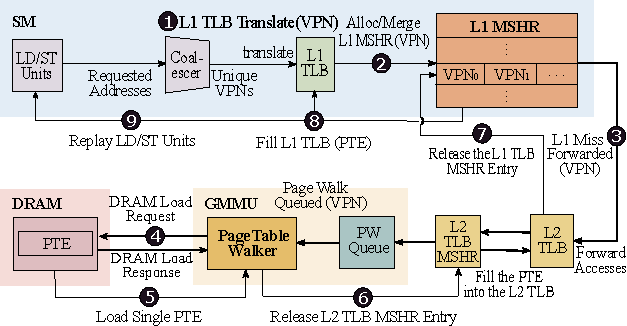
\includegraphics[width=\figwidth]{figs/fig02_TLB_diagram.pdf}
  \caption{GPU address translation hierarchy (SM86): L1 TLB per SM, shared L2 TLB,
  16 PTWs, and MSHR merging for same-VPN requests.}
  \label{fig:arch}
\end{figure}

Figure~\ref{fig:arch} shows the pipeline. Each SM hosts a private, fully-associative
32-entry L1 TLB~\cite{pichai_gpu_translation,translation_cpu}, flushed at kernel boundaries; on the
Ampere SM86 microarchitecture~\cite{nvidia_ampere} studied here, 46 SMs
operate independently. An L1 miss allocates an MSHR entry; a second request
for the same in-flight VPN merges into it rather than issuing a duplicate
walk, and both requestors unblock together on fill. Unmerged L1 misses
forward to the shared, chip-wide L2 TLB (1024 entries on SM86, servicing all
46 SMs), which performs the same same-VPN merge before dispatching to one
of 16 hardware page-table walkers (PTWs)~\cite{shin_irregular}, each
traversing the page table via sequential DRAM reads at hundreds to over a
thousand cycles. With 4\,KB pages, 1024 L2 entries give $4\,\text{MB}$ of
reach; footprints beyond that miss regardless of replacement policy.
Because only 16 PTWs exist, arriving misses queue behind occupied walkers,
and because the L2 MSHR merges by VPN, a single eviction that many warps
depend on stalls all of them at once when re-walked -- the mechanism
behind both the disproportionate cost of a dead-entry miss and the
disproportionate recovery from protecting one. This PTW bottleneck is the
primary reason TLB behavior dominates performance in translation-sensitive
GPU workloads~\cite{pichai_gpu_translation,avoiding_tlb,latpc}.

\subsection{Dead-Entry TLB Misses}

We define a \emph{dead-entry TLB miss} formally:

\begin{center}
\fbox{\begin{minipage}{0.92\columnwidth}
\smallskip
\emph{A TLB miss at virtual page $p$ at time $t$ is a \textbf{dead-entry miss} if $p$
was previously installed in the TLB, subsequently evicted before time $t$, and the
eviction preceded the miss without any intervening access to $p$ that would have
re-established a valid entry.}
\smallskip
\end{minipage}}
\end{center}

\noindent Equivalently, the page-table walker reconstructs a translation that was valid
and present within the current execution window, then discarded by LRU
replacement~\cite{lru,belady} -- the walk is logically redundant, not new
or stale. The classical three-C taxonomy~\cite{hill_smith_3c} describes
\emph{why} an eviction occurred; dead-entry is orthogonal, describing
\emph{what} the evicted entry was, and can arise from either a capacity
eviction (working set exceeds reach) or an interference-driven eviction (a
burst of other pages displaces a still-needed entry) -- the two root
causes behind the workload classes of Section~\ref{sec:characterization}.
Not every capacity or conflict eviction produces a dead-entry event: a
page never re-accessed within the execution window produces no re-walk.
This orthogonality is what makes dead-entry misses actionable where cold
and capacity misses are not: a cold miss needs prediction, a capacity miss
needs more reach, but a dead-entry miss is avoidable in principle simply
by remembering the recent eviction and protecting the re-installed entry
from immediate re-eviction -- the observation that motivates DEPOT.

\section{Related Work}
\label{sec:related}

\noindent\textbf{TLB prefetching and compaction.} LatPC~\cite{latpc} pairs a
stride predictor~\cite{kandiraju_distance} with entry compaction to prefetch
ahead of demand misses; Valkyrie~\cite{valkyrie} and SnakeByte~\cite{snakebyte}
extend stride-based prefetching with multi-level and recursive page-merging
variants. On CPUs, translation-triggered prefetching~\cite{bhattacharjee_ttp}
operates similarly. All predict future translations from access history; we
instead characterize misses by eviction history, an orthogonal signal.

\noindent\textbf{Page-walk optimization.} R2D2~\cite{r2d2} exploits per-warp
address linearity to eliminate redundant walks; Heliostat~\cite{heliostat}
repurposes ray-tracing hardware for parallel walks; SpecTLB~\cite{pham_spectlb}
speculates ahead of confirmed translations. These reduce the \emph{cost} of
walks that occur; we identify a complementary class where the walk itself is
redundant.

\noindent\textbf{Huge pages and page-table layout.} Mosaic~\cite{mosaic}
provides range-TLB reach without OS support; CoLT~\cite{colt} uses contiguous
entries at 4\,KB granularity; Translation Ranger~\cite{translation_ranger}
provides OS support for contiguity-aware TLBs. These address the capacity
limit directly; we use 2\,MB pages only as a diagnostic to separate
capacity-driven from interference-driven misses.

\noindent\textbf{TLB-aware scheduling and dead-block prediction.} CTA
scheduling~\cite{cta_schedule} and MASK~\cite{avoiding_tlb} improve locality
and multi-application concurrency -- these reduce miss \emph{frequency}
through scheduling, whereas our structural cause persists regardless.
Dead-block prediction has a long cache lineage~\cite{rrip,hawkeye}; closest to
our work, Mazumdar et al.~\cite{dop_hpca21} jointly predict dead pages and
blocks via PC-based reuse. We instead use eviction history, requiring no PC
tracking, and quantify prevalence across 24 GPU workloads -- a structurally
distinct miss class not previously isolated at the GPU L2 TLB.

\noindent\textbf{MSHR and CPU TLB characterization.} MSHR occupancy is known
to carry workload-classification signal for cache/memory
tuning~\cite{mshr_mgmt}; we apply an analogous signal to the TLB MSHR. CPU TLB
studies~\cite{translation_cpu} attribute misses mainly to working-set
overflow; GPUs differ in that thousands of concurrent warps interact through
one shared L2 TLB and MSHR, producing amplification effects absent on CPUs.

\section{Methodology}
\label{sec:methodology}

\subsection{Simulation Platform}

All experiments run on Accel-Sim~\cite{accelsim}, a cycle-accurate GPU simulator
built on GPGPU-Sim~\cite{gpgpusim}.
We adopt Accel-Sim's default \texttt{SM86\_RTX3070} configuration~\cite{accelsim},
which models an NVIDIA GeForce RTX~3070-class GPU~\cite{rtx3070} based on the Ampere
microarchitecture~\cite{nvidia_ampere,ampere_microbench}; the baseline GPU, cache, and
memory parameters are used unmodified.
The TLB hierarchy parameters---L1 and L2 TLB capacities, MSHR depths, lookup latencies,
and the 16 page-table walkers---follow the configuration used in the state-of-the-art work~\cite{latpc},
ensuring our results are directly comparable to that prior work.
Table~\ref{tab:tlb_config} summarizes the configuration.
The L2 TLB has 1024 entries with LRU replacement, providing 4\,MB of reach with 4\,KB pages.
Page-table walks are modeled with 16 dedicated PTWs, each capable of one concurrent walk.
The L2 MSHR supports 128 in-flight translation requests; same-VPN requests are merged
into a single MSHR entry.


\begin{table}[ht]
  \centering
  \caption{Simulated System Configuration.}
  \label{tab:tlb_config}
  \scriptsize
  \setlength{\tabcolsep}{4pt}
  \renewcommand{\arraystretch}{1.2}
  \begin{tabular}{|>{\centering\arraybackslash}m{0.14\columnwidth}|m{0.74\columnwidth}|}
    \hline
    \multicolumn{2}{|c|}{\textbf{GPU Configuration}} \\
    \hline
    SM & 46 SMs, 1536 threads / 32-thread warps, 32 CTAs per SM\newline
         65{,}536 registers per SM, up to 100\,KB shared memory\newline
         1132\,MHz core clock \\
    \hline
    Cache & 128\,B line; L1 D-cache 128\,KB, 32-way, 384 MSHRs\newline
            L2 cache (unified) 4\,MB, 16-way \\
    \hline
    DRAM & GDDR6, 16 channels, 14\,Gbps, 3500.5\,MHz\newline
           254-cycle access latency \\
    \hline
    % Interconnect & iSLIP arbiter, 2 subnets, 40\,B flit \\
    \hline
    \multicolumn{2}{|c|}{\textbf{Virtual Memory Configuration}} \\
    \hline
    L1 TLB & 32 entries, fully associative, 4\,KB pages\newline
             16 MSHRs (4-way merge), 4 ports\newline
             20-cycle lookup latency, LRU replacement \\
    \hline
    L2 TLB & 1024 entries, 16-way, 4\,KB pages\newline
             128 MSHRs (8-way merge), 16 ports\newline
             80-cycle lookup latency, LRU replacement\newline
             Reach 4\,MB (4\,KB) / 256\,MB (2\,MB pages) \\
    \hline
    Page Walk & 16 page-table walkers\newline
                x86-64 4-level page table~\cite{amd64_manual,intel_sdm},
                254 cycles per level\newline
                32-entry page-walk cache, 20-cycle lookup \\
    \hline
  \end{tabular}
\end{table}

\subsection{Instrumentation}

We extend Accel-Sim with four measurement modules: a \emph{miss arrival timeseries}
recording every L2 TLB miss's arrival timestamp; \emph{dead-entry detection}, which
tracks the last eviction cycle per VPN in a hash table and classifies a miss as
dead-entry if the VPN appears there; an \emph{MSHR dead-slot timeseries}, sampling at
100-cycle intervals the number of MSHR entries awaiting dead-entry re-walks, whose peak
defines the \emph{burstiness} metric; and \emph{DEPOT protection statistics} (Bloom
filter insert/hit counts, protected-entry counts, LRU fallback events; implementation
details in Section~\ref{sec:depot}).

\subsection{Workload Suite}
Table~\ref{tab:workloads} characterizes all 24 workloads
(Classes: \textbf{A}\,=\,interference-driven; \textbf{B}\,=\,capacity-driven; \textbf{---}\,=\,not TLB-sensitive). Here, MPKI is L2 TLB misses per kilo-instruction, while mem-MPKI is misses per
kilo memory-instruction, isolating translation pressure from non-memory compute.
We select applications with working sets exceeding 4\,MB or L2 TLB MPKI above 1.0,
matching the criteria used in LatPC~\cite{latpc}.
Workloads span Rodinia~\cite{rodinia}, PolyBench~\cite{polybench}, Lonestar~\cite{lonestar},
Parboil~\cite{parboil}, and Pannotia~\cite{pannotia} benchmark suites.
We apply a two-bin framing: \textbf{TLB-sensitive} workloads (L2 MPKI $\geq 1$, matching the
selection criterion of LatPC~\cite{latpc}) vs.\ \textbf{not TLB-sensitive} workloads
(L2 MPKI $< 1$).
Nine workloads meet the TLB-sensitive threshold (including \texttt{mst} at MPKI$\,{=}\,0.98$,
a near-threshold borderline case with confirmed capacity-driven root cause);
the remaining 15 serve as a graceful-degradation validation set.
Within the TLB-sensitive bin, we sub-classify by access structure:
\textbf{Class~A} (interference-driven) for workloads where all threads in a warp
reference the same virtual page (shared VPN)---producing MSHR-merge amplification---and
\textbf{Class~B} (capacity-driven) for workloads where each warp instruction generates
distinct VPNs per thread, driving working-set-overflow evictions that exceed TLB reach.
Class~B membership is confirmed by the 2\,MB IPC experiment: if switching to 2\,MB pages
(L2 reach $= 256$\,MB) yields a large IPC speedup, the workload was reach-limited.


\begin{table}[t]
  \centering
  \caption{List of Evaluated Workloads.}
  \label{tab:workloads}
  \scriptsize
  \setlength{\tabcolsep}{4pt}
  \renewcommand{\arraystretch}{1.05}
  \begin{tabular}{@{}llrrrc@{}}
    \toprule
    \textbf{Workload} & \textbf{Suite} & \textbf{MPKI} & \textbf{mem-MPKI} & \textbf{Footprint} & \textbf{Cls} \\
    \midrule
    atax            & PolyBench & 81.4   & 119.6  & 16.0\,MB   & A \\
    mvt               & PolyBench & 56.5   & 83.0   & 16.0\,MB   & A \\
    \midrule
    bicg            & PolyBench & 56.4   & 82.8   & 16.0\,MB   & B \\
    gesummv           & PolyBench & 175.5  & 249.7  & 31.3\,MB   & B \\
    nw                  & Rodinia   & 5.02   & 67.9   & 32.0\,MB   & B \\
    dmr                  & Lonestar  & 2.99   & 18.6   & 24.2\,MB   & B \\
    kmeans              & Rodinia   & 2.09   & 72.5   & 30.3\,MB   & B \\
    sssp           & Lonestar  & 1.58   & 11.3   & 48.0\,MB   & B \\
    mst                & Lonestar  & 0.98   & 6.80   & 73.0\,MB   & B \\
    \midrule
    backprop          & Rodinia   & 0.02   & 0.30   & 9.0\,MB    & --- \\
    bfs                & Rodinia   & 0.03   & 0.20   & 2.4\,MB    & --- \\
    gaussian            & Rodinia   & 0.00   & 0.01   & 0.5\,MB    & --- \\
    hybridsort          & Rodinia   & 0.02   & 0.46   & 12.0\,MB   & --- \\
    lud                 & Rodinia   & 0.03   & 0.58   & 16.0\,MB   & --- \\
    pagerank                  & Pannotia  & 0.06   & 0.40   & 10.9\,MB   & --- \\
    p-bfs                & Parboil   & 0.00   & 0.07   & 1.1\,MB    & --- \\
    mri-gridding         & Parboil   & 0.09   & 6.04   & 226.4\,MB  & --- \\
    sad                       & Parboil   & 0.02   & 1.48   & 8.5\,MB    & --- \\
    sgemm               & Parboil   & 0.00   & 0.07   & 12.0\,MB   & --- \\
    spmv                      & Parboil   & 0.19   & 0.71   & 29.4\,MB   & --- \\
    2mm            & PolyBench & 0.00   & 0.00   & 5.0\,MB    & --- \\
    fdtd2d          & PolyBench & 0.09   & 0.49   & 48.0\,MB   & --- \\
    gramschmidt               & PolyBench & 0.40   & 0.62   & 24.4\,MB   & --- \\
    streamcluster        & Rodinia   & 0.17   & 0.70   & 8.4\,MB    & --- \\
    \bottomrule
  \end{tabular}
\end{table}


\subsection{Evaluated Configurations}

We evaluate six configurations: (i) Baseline: Unmodified LRU replacement, 4\,KB pages, (ii) DEPOT: DEPOT eviction protection enabled with default parameters ($W = 500\text{K}$ cycles, 8192-bit Bloom filter), (iii) 2\,MB baseline: Baseline with 2\,MB huge pages (L2 TLB reconfigured to 128 entries $\times$ 2\,MB, reach = 256\,MB), (iv) 2\,MB+DEPOT: DEPOT with 2\,MB pages, (v) LatPC: State-of-the-art TLB prefetching and compaction~\cite{latpc} enabled, 4\,KB pages, and (vi) LatPC+DEPOT: Both LatPC and DEPOT enabled simultaneously.

\section{Dead-Entry Miss Characterization}
\label{sec:characterization}

\subsection{Dead-Entry Ratio}
\label{sec:char_de_ratio}

Dead-entry misses are not a rare edge case but the dominant miss type across the
suite: 16 of 24 workloads exhibit dead-entry ratios above 90\%, and all 9
TLB-sensitive workloads exceed 98\% (six above 99\%). This near-unity ratio arises
because a TLB-sensitive workload's working set is large enough to force eviction
between successive accesses to the same page, yet small enough that the same
pages recur within a kernel -- so virtually every steady-state L2 miss re-walks a
page the TLB has already translated and discarded. High DE ratio alone does not
imply TLB sensitivity, however: \texttt{lud} and \texttt{gramschmidt} exceed 99\%
DE ratio yet sustain high throughput because their absolute miss rate is too low
for cumulative stall time to matter, motivating a joint condition of high DE
ratio \emph{and} high MPKI.

\begin{figure}[t]
  \centering
  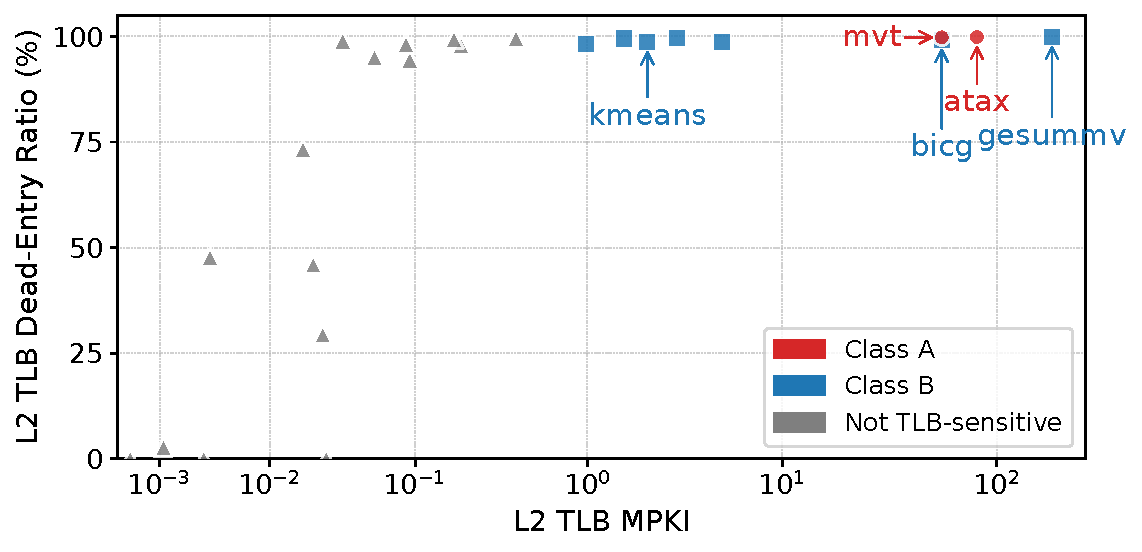
\includegraphics[width=\figwidth]{figs/fig04_de_ratio_vs_mpki.pdf}
  \caption{L2 TLB Dead-entry ratio vs.\ L2 TLB MPKI for all 24 workloads.}
  \label{fig:de_mpki}
\end{figure}

Figure~\ref{fig:de_mpki} plots all 24 workloads by DE ratio against MPKI. A
vertical gap separates the 9 TLB-sensitive workloads, at elevated MPKI, from the
other 15, and within that high-MPKI band every workload clusters near 100\% DE
ratio -- confirming near-unity DE ratio as a reliable marker of TLB-sensitive
steady state. Below the gap, DE ratio spans near-zero to above 99\% with no
relation to MPKI, confirming it carries no predictive power on its own.

\subsection{Access Structure: The Class Discriminator}
\label{sec:char_burstness}

\texttt{atax} and \texttt{bicg} illustrate why miss statistics alone are
insufficient: they share nearly identical DE ratios ($\sim$99.9\%/$\sim$99.2\%)
and comparable MPKI (81/56), and even their miss arrival rates track closely
through steady state, yet their response to the same eviction-history protection
differs by nearly two orders of magnitude. The discriminator is access
structure -- whether warps reference the same virtual page or distinct pages at
a given moment -- and Figure~\ref{fig:burstness} makes it visible directly:
\texttt{atax} shows brief, high-amplitude occupancy bursts, while \texttt{bicg}
is flat and sustained throughout.

\begin{figure}[ht]
  \centering
  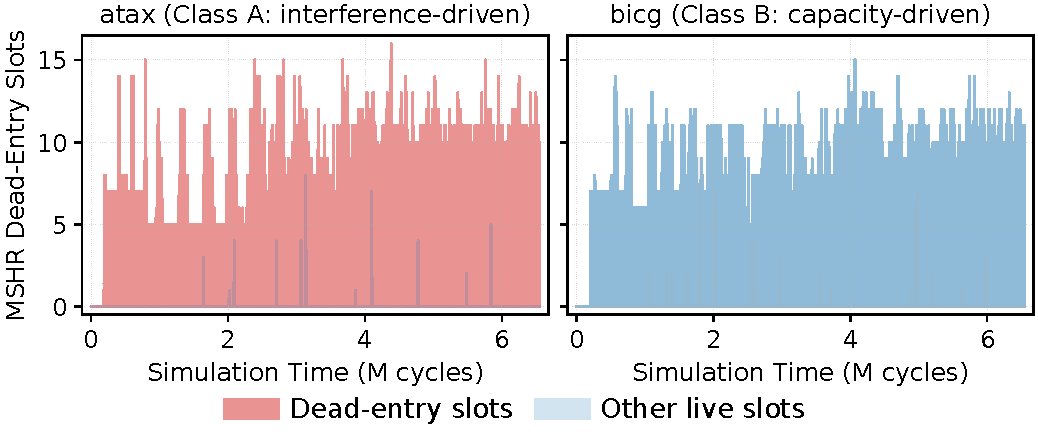
\includegraphics[width=\figwidth]{figs/fig06_mshr_burstness.pdf}
  \caption{MSHR dead-slot occupancy over time for \texttt{atax} and \texttt{bicg}.}
  \label{fig:burstness}
\end{figure}

In \texttt{atax}, each warp computes $y \mathrel{+}= A[i][j] \cdot x[j]$: all 32
threads access the same element of $x[]$, producing one shared VPN per warp
instruction. When that VPN is evicted and re-walked, every warp stalled on it
merges into a single MSHR entry, so one page walk releases many warps at once,
producing the sharp spikes in Figure~\ref{fig:burstness} (spike height tracks
merge depth); \texttt{mvt} shares this pattern for analogous algebraic reasons,
forming Class~A's second member. In \texttt{bicg}, each warp computes a column
dot product where thread $i$ accesses row $i$ of $A$, producing 32 distinct VPNs
per warp instruction with a merge depth near one -- its 2048-by-2048 working set
needs $\sim$4096 pages, four times L2 TLB capacity, so evictions are
capacity-driven and the occupancy trace stays flat, a structure shared by the
remaining six Class~B workloads (\texttt{nw}, \texttt{sssp}, \texttt{kmeans},
\texttt{gesummv}, \texttt{dmr}, \texttt{mst}). The two classes are thus
distinguished by occupancy shape alone -- bursty spikes mean shared pages and
disproportionate per-eviction recovery, flat sustained occupancy means
capacity-bound evictions no replacement policy can resolve -- observable from
existing MSHR counters with no offline profiling required.

\subsection{Validating Capacity-Driven Misses}
\label{sec:char_2mb}

If the seven Class~B workloads are genuinely capacity-driven, expanding TLB
reach should eliminate their dead-entry misses. Figure~\ref{fig:de_2mb} shows
IPC speedup under 2\,MB huge pages (L2 reach $4\,\text{MB}\rightarrow256\,\text{MB}$)
over the 4\,KB baseline for all nine TLB-sensitive workloads.

\begin{figure}[ht]
  \centering
  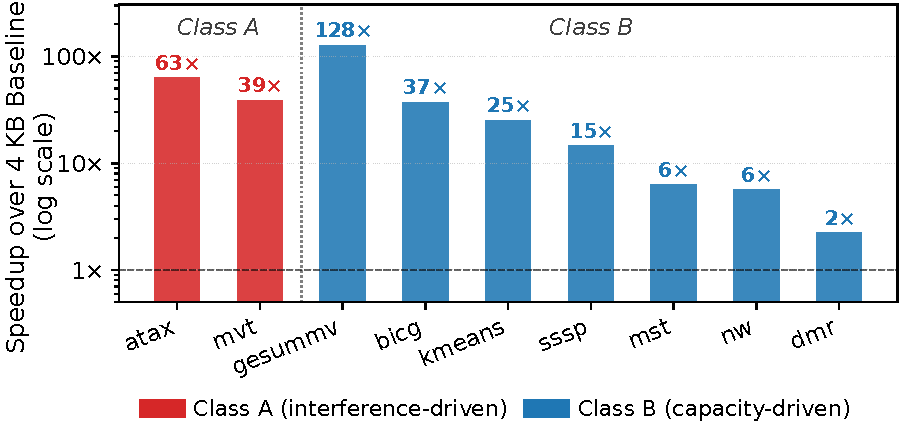
\includegraphics[width=\figwidth]{figs/fig07_2mb_ipc_speedup.pdf}
  \caption{IPC speedup under 2\,MB pages over 4\,KB baseline for all 9 TLB-sensitive workloads.}
  \label{fig:de_2mb}
\end{figure}

Results confirm the diagnosis for all 7 Class~B workloads, with speedups
tracking working-set size relative to the expanded reach: \texttt{gesummv}
$128\times$ (16\,MB set fits entirely), \texttt{bicg} $37\times$, \texttt{kmeans}
$25\times$, \texttt{sssp} $14.5\times$, \texttt{mst} $6.3\times$, \texttt{nw}
$5.7\times$, and \texttt{dmr} $2.2\times$ (a more irregular address stream, only
partially contained). Class~A also benefits substantially (\texttt{atax}
$63\times$, \texttt{mvt} $39\times$), but unlike Class~B, its performance is not
fundamentally capacity-constrained -- expanding reach does not eliminate the
interference among warps competing for the same entries.

\section{DEPOT: Dead-Entry PrOTection}
\label{sec:depot}

%\subsection{Mechanism Design}
%\label{sec:o3_mech}

In this section, we propose DEPOT that targets Class~A dead-entry re-walks through a three-phase mechanism
detection, fill, and eviction implemented entirely within the L2 TLB
pipeline. Figure~\ref{fig:depot_mech} shows the hardware. Three additions extend the
existing L2 TLB datapath: an eviction-history Bloom filter, a small Pending
Dead-Entry Set (PDS) that bridges the miss and fill events, and a Protection
Timestamp Writer that drives a new 20-bit per-entry protection-timer field in
the tag array.

\begin{figure}[ht]
  \centering
  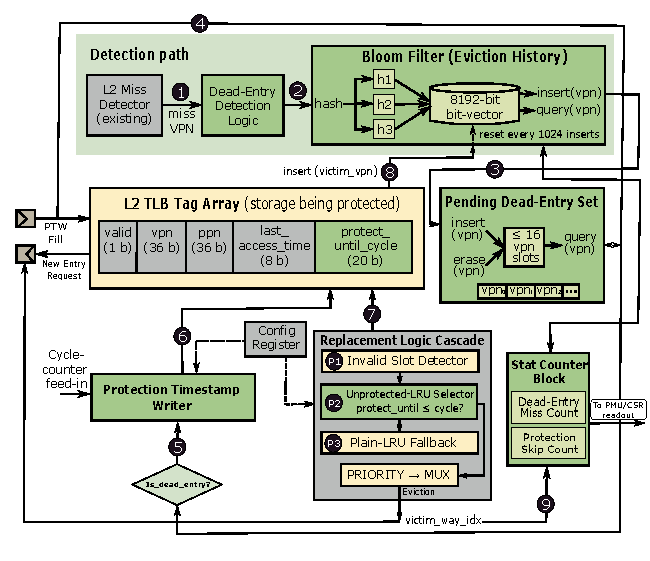
\includegraphics[width=\columnwidth]{figs/fig8_DEPOT_mechanism_long.pdf}
  \caption{DEPOT mechanism: eviction-history Bloom filter, Pending
  Dead-Entry Set, per-entry protection timer, and protection-aware
  replacement cascade.}
  \label{fig:depot_mech}
\end{figure}

\noindent\textbf{Detection (miss path).}
On every L2 TLB miss, the Dead-Entry Detection Logic receives the missed
VPN~\circnum{1} and hashes it through three independent hash functions
($h_1, h_2, h_3$) into an 8192-bit Bloom filter~\cite{bloom_filter} that records recently
evicted VPNs~\circnum{2}.
A filter hit indicates that the missed VPN was recently in the TLB and is
therefore a probable dead-entry re-walk, so the in-flight miss is registered
in the PDS~\circnum{3}-a small ($\le 16$ slot) buffer that holds VPNs
awaiting fill.
Misses whose VPN is absent from the filter (genuine cold or capacity misses
with no eviction history) bypass the PDS and proceed through the standard
page-walk path.

\noindent\textbf{Fill (protection path).}
When the page-table walk completes, the fill triggers a PDS query for the
filling VPN~\circnum{4}.
A PDS hit activates the Protection Timestamp Writer~\circnum{5}, which
reads the cycle counter and sets the newly installed entry's protection
timer to expire at $\textit{now} + W$ cycles~\circnum{6}, where $W$
defaults to 500\,K cycles and is held in a configuration register.
The PDS slot for that VPN is then released.
Fills whose VPN was not previously flagged install with the protection field
untouched and behave identically to baseline.

\noindent\textbf{Eviction (protection-aware replacement).}
On every fill that requires a victim, the Replacement Logic Cascade reads
each entry's protection timer from the tag array~\circnum{7} and selects
through three priority stages:
\emph{\circnum{P1}~Invalid Slot Detector} returns any invalid entry immediately;
\emph{\circnum{P2}~Unprotected-LRU Selector} compares each entry's protection timer
against the current cycle and selects the LRU entry among those whose
protection has expired;
\emph{\circnum{P3}~Plain-LRU Fallback} fires only when every candidate in the set is
still protected, in which case the cascade reverts to standard LRU.
The selected victim's VPN is inserted into the Bloom filter, refreshing the
eviction history~\circnum{8}, and the victim's way index is forwarded to
a small Stat Counter Block~\circnum{9} that records dead-entry-miss and
protection-skip counts.
This graceful degradation is a correctness property: it bounds the worst-case
overhead of DEPOT to zero, since the fallback path is indistinguishable from
baseline LRU. Two operational details keep the mechanism stable across long-running workloads.
First, the filter is reset after every 1024 insertions rather than on a fixed
time interval; this count-based threshold keeps the expected false-positive rate
below 5\% while avoiding the temporal aliasing of a cycle-timer reset that could
misfire across kernel boundaries.
Second, a protection-state flush at each kernel boundary clears all protection
timers, ensuring that a VPN evicted during kernel $K_n$ does not spuriously
protect an entry in kernel $K_{n+1}$, where the same virtual address may map to
a different physical frame after relaunch.

Regarding hardware cost, the Bloom filter occupies 1\,KB of storage.
Each TLB entry requires one additional per-entry protection timer of 20 bits to record
the expiry cycle, yielding $1024 \times 20 = 20\,\text{Kbits} = 2.5\,\text{KB}$ of
per-entry SRAM across the full 1024-entry L2 TLB.
The total overhead is therefore $1\,\text{KB} + 2.5\,\text{KB} = 3.5\,\text{KB}$,
amortized across the existing TLB array. DEPOT's eviction-history Bloom filter is structurally similar to the evicted-address
filter introduced by Seshadri et al.~\cite{evicted_addr_filter} for cache pollution and
thrashing mitigation; we apply the same primitive at the TLB layer, where eviction-history
information drives protection rather than insertion policy.

\section{Performance Evaluation and Analysis}
\label{sec:evaluation}

\subsection{DEPOT Performance}
\label{sec:o3_real}

\begin{figure}[t]
  \centering
  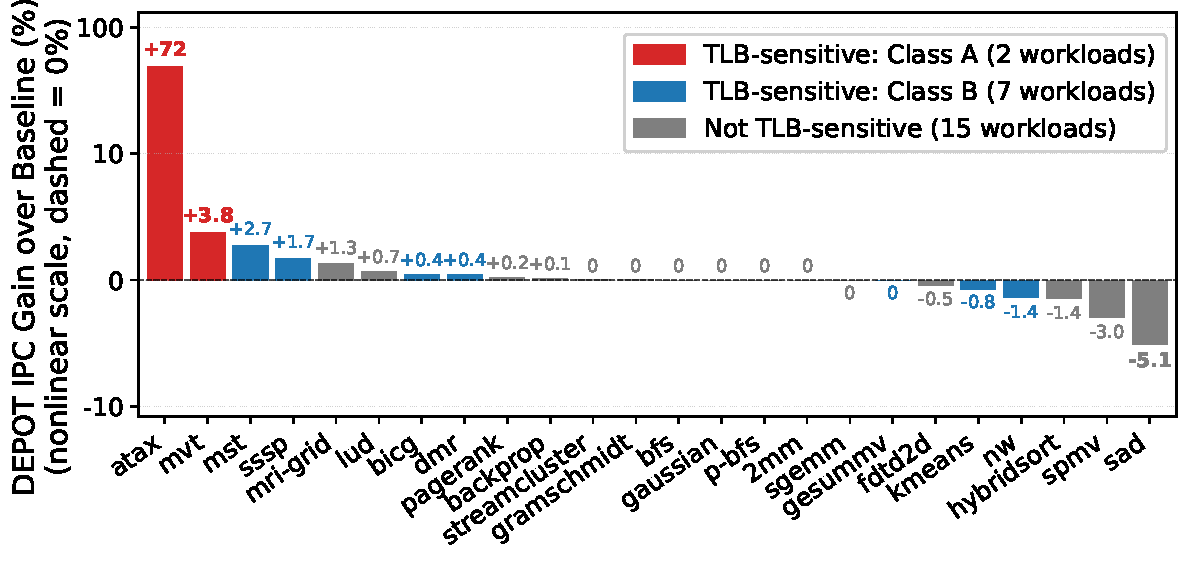
\includegraphics[width=\figwidth]{figs/fig09_o3_ipc_gains.pdf}
  \caption{IPC improvement of DEPOT over 4\,KB baseline for all 24 workloads, sorted descending.}
  \label{fig:o3_gains_bar}
\end{figure}

Figure~\ref{fig:o3_gains_bar} shows IPC improvement of DEPOT for all 24 workloads.
The results divide cleanly along the class boundaries established in
Section~\ref{sec:characterization}.
Among the 15 not-TLB-sensitive workloads, IPC improvement is near zero throughout, with
occasional small negative values including \texttt{sad} at $-5.1\%$ and \texttt{spmv}
at $-2.9\%$.
These minor regressions arise because DEPOT occasionally fires on workloads with
moderate DE ratios, marking re-installed entries as protected even though TLB misses
are not on their critical path; with MPKI of 0.02 and 0.19 respectively,
\texttt{sad} and \texttt{spmv} incur negligible TLB stall time at baseline,
so the observed losses reflect second-order LRU displacement rather than
translation overhead.
The LRU fallback bounds worst-case degradation but activates only when all entries
in a set are simultaneously protected, so partial-protection sets can still make
suboptimal eviction choices, which accounts for the small residual regression.
% These minor regressions arise from interactions between the modified replacement policy
% and moderate-DE-ratio workloads where the Bloom filter marks entries that are not
% performance-critical, slightly shifting eviction pressure onto others.
% In all 15 cases the workloads operate at the normalized IPC of well above 1.0, so the absolute cycle
% impact is negligible, and the LRU fallback limits worst-case degradation by design.
Among the two Class~A workloads, \texttt{atax} improves from 0.354 to 0.610 IPC for
a gain of $+72\%$, reflecting near-complete elimination of dead-entry re-walk stalls
that previously dominated its execution time.
\texttt{mvt} improves from 0.574 to 0.596 IPC for a gain of $+3.8\%$.
The smaller gain on \texttt{mvt} reflects its peak MSHR merge depth of 15 versus
\texttt{atax}'s 17 and its higher baseline IPC, indicating that TLB stalls already
represent a smaller fraction of its execution time before DEPOT is applied.
Both workloads converge to similar post-DEPOT IPC values near 0.60, consistent with
reaching a shared performance ceiling determined by compute throughput and memory
bandwidth rather than translation overhead.
All seven Class~B workloads show near-zero DEPOT gain, ranging from $-1.4\%$ to
$+2.7\%$, within simulation noise. This result holds across PolyBench, Lonestar, and Rodinia workloads: when each warp generates distinct VPNs, protecting one re-installed entry is immediately offset by another capacity eviction, while the LRU fallback ensures zero overhead.
\begin{comment}
All seven Class~B workloads show near-zero DEPOT gain, ranging from $-1.4\%$ to
$+2.7\%$, all within simulation noise. The result holds uniformly across PolyBench dense linear algebra, Lonestar graph workloads, and Rodinia clustering benchmarks: whenever each warp instruction generates
distinct VPNs, protecting any individual re-installed entry is immediately offset by a
new capacity eviction elsewhere, and the LRU fallback ensures zero overhead.
\end{comment}

\begin{figure}[ht]
  \centering
  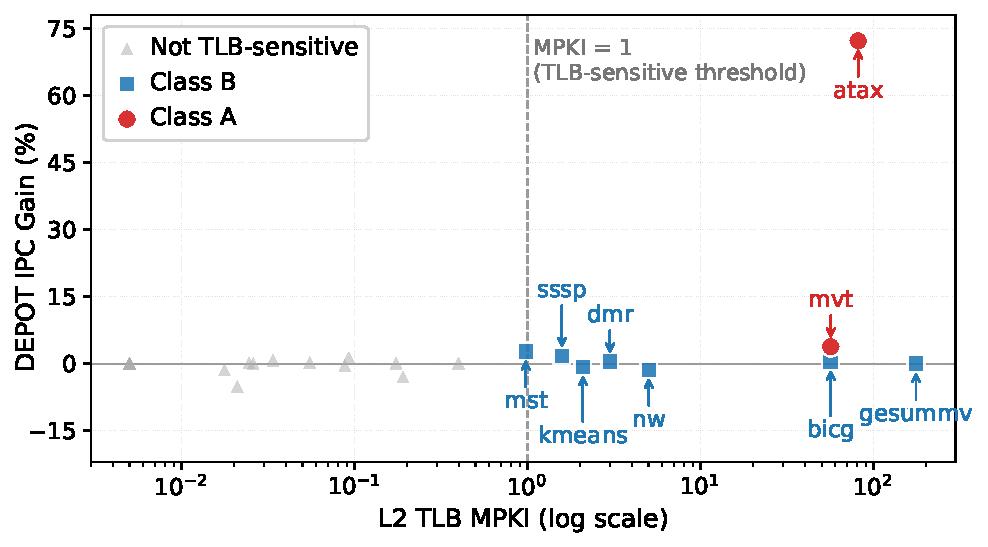
\includegraphics[width=\figwidth]{figs/fig11_o3gain_vs_mpki.pdf}
  \caption{IPC improvement of DEPOT vs.\ L2 TLB MPKI for all 24 workloads.}
  \label{fig:o3_scatter}
\end{figure}

Figure~\ref{fig:o3_scatter} plots IPC improvement of DEPOT against MPKI for all 24 workloads,
revealing a clean two-regime structure.
Workloads with MPKI below 1 cluster near zero gain regardless of their dead-entry ratio,
confirming that TLB miss rate is a necessary condition for sensitivity.
Within the high-MPKI group, workloads split by access structure: those with shared VPN
access show positive gains, while those with unique VPN access per warp show near-zero
gains.
The scatter plot makes visible what the aggregate bar chart in
Figure~\ref{fig:o3_gains_bar} obscures: MPKI identifies workloads for which TLB
behavior matters at all, while access structure determines whether eviction-history
protection can improve it.
To bound the overhead from false positives, we also evaluate a worst-case scenario with
a fully saturated Bloom filter, where every miss query returns a positive response
regardless of actual eviction history.
Under saturation, \texttt{atax} IPC remains at 0.610, identical to the normal DEPOT
result.
False positives cause DEPOT to protect entries that did not originate from dead-entry
re-walks, but the LRU fallback absorbs the resulting mismatch without measurable
performance impact, showing that the mechanism is tolerant of false positive pressure.

\begin{figure}[ht]
  \centering
  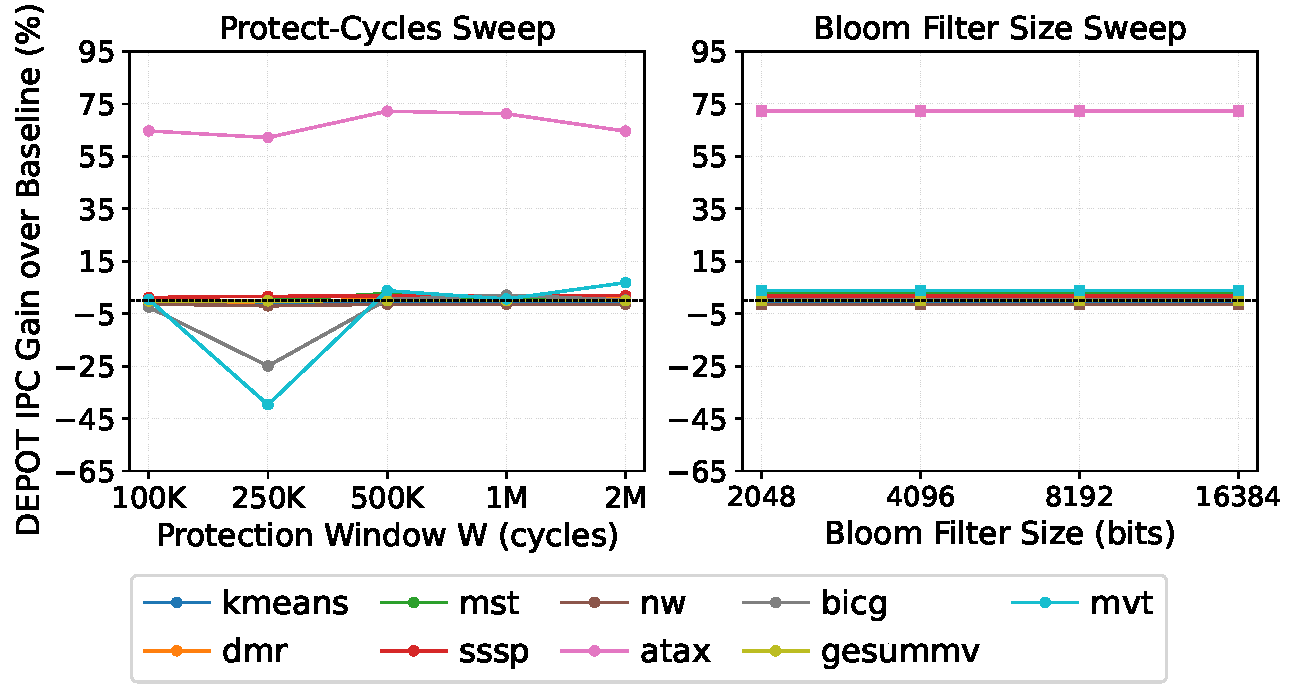
\includegraphics[width=\figwidth]{figs/fig13_param_sensitivity.pdf}
  \caption{DEPOT parameter sensitivity for 9 TLB-sensitive workloads: protection window $W$ (left) and Bloom filter size (right).}
  \label{fig:params}
\end{figure}

Figure~\ref{fig:params} shows DEPOT sensitivity to its two configurable parameters for 9 TLB-sensitive workloads. Both the protection-window sweep (100\,K to 2\,M) and Bloom-filter sweep (2048 to 16384 bits) remain nearly flat across the tested range. This indicates that TLB-sensitive workloads experience re-walk bursts within timescales covered by any reasonable protection window, while the eviction stream remains well below the saturation threshold of even the smallest Bloom filter. DEPOT is therefore robust to parameter choice, and the default configuration of a 500\,K-cycle protection window and an 8192-bit Bloom filter is effective across all evaluated workloads without tuning.

\begin{comment}
Figure~\ref{fig:params} shows the sensitivity of DEPOT to its two configurable
parameters for 9 TLB-sensitive workloads.
Both the protection window and the Bloom filter size sweeps are flat across the full
tested range, with the window varying from 100\,K to 2\,M cycles and the filter size
varying from 2048 to 16384 bits.
The insensitivity to window size reflects that TLB-sensitive workloads experience
re-walk events on timescales short enough that any reasonable protection duration covers
the relevant burst interval, so extending or shortening the window produces no
measurable change.
The insensitivity to filter size reflects that the eviction stream of TLB-sensitive
workloads is well below the saturation threshold of even the smallest tested
configuration, so adding more bits provides no additional discriminating power.
DEPOT is therefore robust to parameter choice, and the default configuration of a
500\,K-cycle protection window and an 8192-bit Bloom filter is safe across all
workloads tested without tuning.
\end{comment}

\subsection{Class~A/B Asymmetry}
\label{sec:disc_classes}
The performance asymmetry between Class A and Class B follows directly from the access-structure analysis in Section~\ref{sec:char_burstness} and explains both the large gains on \texttt{atax} and the near-zero results on the Class B workloads. In Class A workloads, a single dead-entry eviction is amplified through MSHR merging because many warps simultaneously reference the same virtual page. When DEPOT protects the re-installed entry, it eliminates both the initial re-walk and the merged re-walks that would otherwise stall many warps simultaneously. On SM86, page-walk latency is approximately 300–500 cycles, and releasing dozens of stalled warps with a single protection event can recover thousands of cycles, consistent with the observed +72\% IPC improvement.

In Class B workloads, by contrast, the TLB is continuously occupied by a working set that exceeds TLB reach, and each warp accesses distinct pages with little cross-warp sharing. Protecting one re-installed entry therefore only shifts the next eviction to another entry without reducing the overall eviction rate. Because MSHR merging is minimal, each page walk serves only one warp, so the benefit of protection is limited. When all entries are under protection pressure, DEPOT falls back to standard LRU replacement, ensuring negligible overhead in this regime.

\begin{comment}
The performance asymmetry between Class~A and Class~B follows directly from the access
structure analysis in Section~\ref{sec:char_burstness}, and understanding it explains
both the large gains on \texttt{atax} and the near-zero results on the Class~B workloads.
In Class~A workloads, a single dead-entry eviction is not an isolated event: because
many warps simultaneously reference the same virtual page, that eviction stalls all of
them at once through the MSHR merge mechanism.
When DEPOT protects the re-installed entry, it remains in the TLB through the entire
burst of warp accesses referencing that page, eliminating not just the first re-walk
but all of the merged re-walks in the burst simultaneously.
The result is that one protection decision avoids many stall cycles, and the compounding
effect is what produces the large observed IPC gain on \texttt{atax}.
The page-walk latency to DRAM on the SM86 microarchitecture is approximately 300 to
500 cycles, and when a burst of dozens of warps is unblocked by a single protection
event, the total recovered cycles per event can reach into the thousands, consistent
with the $+72\%$ IPC improvement observed.
In Class~B workloads, by contrast, the TLB entry pool is fully occupied by the working
set, and each warp accesses distinct pages with no cross-warp sharing.
Protecting one re-installed entry simply forces a different equally-soon-to-be-evicted
entry to absorb the next eviction instead, shifting which entry is displaced without
reducing how many evictions occur overall.
Because there is no MSHR merging, each page walk serves exactly one warp, and
protecting one entry saves at most one page-walk latency before a new capacity eviction
immediately regenerates a dead-entry miss at the same location.
The LRU fallback handles the case where all entries are simultaneously under protection
pressure by yielding to standard LRU, ensuring DEPOT imposes no overhead in this regime.
\end{comment}

\subsection{Composition with LatPC}
\label{sec:o3_latpc}

LatPC combines stride-based prefetching with entry compaction and represents the
state-of-the-art in GPU TLB optimization.
It trains a stride predictor for each TLB entry and issues prefetch requests before
demand misses occur, targeting cold and capacity-driven misses through access-pattern
prediction.
DEPOT and LatPC address fundamentally different sources of TLB misses: LatPC reduces
misses by predicting future accesses and filling the TLB ahead of demand, while DEPOT
reduces misses by preventing recently installed entries from being prematurely evicted
at the replacement boundary.
Because their mechanisms operate on different points in the TLB pipeline, one does not
subsume the other: on interference-driven workloads the two compose additively, while
on capacity-saturated workloads they can contend, as the results below show.

\begin{figure}[ht]
  \centering
  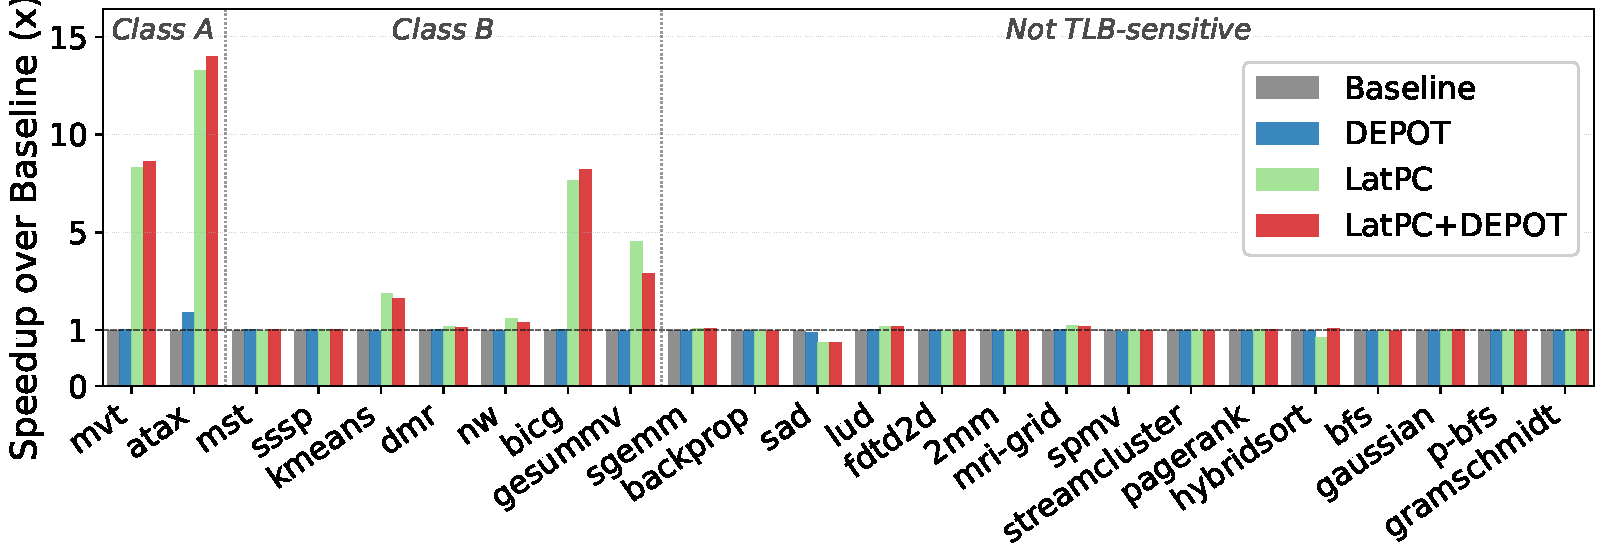
\includegraphics[width=\figwidth]{figs/fig10_ipc_comparison.pdf}
  \caption{IPC comparison across four configurations for all 24 workloads.}
  \label{fig:ipc}
\end{figure}

Figure~\ref{fig:ipc} shows the composition result across all configurations.
LatPC alone achieves large gains on TLB-sensitive workloads, with \texttt{atax}
improving by $+1227\%$ from 0.354 to 4.70\,IPC, \texttt{bicg} by $+667\%$ from 0.601
to 4.61\,IPC, and \texttt{mvt} by $+729\%$ from 0.574 to 4.76\,IPC.
These gains reflect LatPC's elimination of the dominant cold-miss bottleneck, which
accounts for the large majority of TLB stalls in these workloads.
LatPC+DEPOT outperforms LatPC alone on the Class~A workloads, with \texttt{atax}
improving further from 4.70 to 4.95\,IPC ($+5.4\%$) and \texttt{mvt} from 4.76 to
4.95\,IPC ($+4.0\%$).
Across the Class~B workloads, LatPC+DEPOT shows mixed results: \texttt{bicg}
($+6.9\%$), \texttt{mst} ($+2.5\%$), and \texttt{sssp} ($+2.1\%$) gain modestly,
\texttt{dmr} is negligible ($-0.9\%$), while \texttt{kmeans} ($-8.3\%$),
\texttt{nw} ($-10.0\%$), and \texttt{gesummv} ($-28.5\%$) regress.
These regressions arise because DEPOT's eviction-protection policy conflicts with
LatPC's prefetch-driven replacement in capacity-saturated workloads: LatPC must
freely evict entries to install ahead-of-demand translations, and DEPOT's protected
entries block those slots, delaying prefetch fills and causing net IPC loss.

The additive improvement on Class~A workloads arises because LatPC does not eliminate all
dead-entry re-walks even when its prefetcher is operating correctly.
The key reason is the asymmetry between what the prefetcher targets and what eviction
produces.
LatPC observes that a warp accesses VPN $A$, then predicts and prefetches the next
VPN in the stride sequence.
While the prefetch is in flight, VPN $A$ itself may be displaced from the TLB by LRU
replacement, because the prefetch installs a new entry and the LRU policy does not
know that $A$ will be accessed again at the next stride period.
When that next access to $A$ arrives it finds the entry gone, a dead-entry miss that
LatPC's forward-looking predictor cannot catch; DEPOT observes the eviction of $A$
at the replacement boundary and protects the re-installed entry, covering exactly
this residual class.
Where the combination is beneficial---the Class~A workloads and \texttt{bicg}---the
2 to 7\% additional IPC improvement reflects how frequently this interaction between
prefetch-driven installation and LRU displacement produces residual dead-entry events.
The marginal hardware cost of adding DEPOT to a LatPC-equipped TLB is a 1\,KB Bloom
filter, negligible relative to LatPC's per-entry stride prediction tables, making the
combination an efficient pairing for workloads that benefit from both.

\section{Discussion and Limitations}
\label{sec:discussion}

The 2\,MB page results in Section~\ref{sec:char_2mb} raise a natural question about whether
DEPOT is necessary if larger pages already resolve TLB pressure.
The two mechanisms address different root causes and are not interchangeable.
Larger pages expand TLB reach and directly relieve capacity eviction in Class~B workloads,
but they do not eliminate interference-driven eviction in Class~A workloads, nor are they
always available: GPU workloads frequently use custom memory pools or third-party libraries
that do not guarantee 2\,MB alignment, and virtualized environments may not expose huge page
support to guest workloads at all.
DEPOT operates entirely within the TLB microarchitecture and is transparent to the OS,
driver, and application, making it applicable in settings where large pages are unavailable
or impractical.

DEPOT targets interference-driven dead-entry misses and provides no benefit for workloads
whose TLB pressure arises from working-set overflow beyond the TLB reach.
The Class~B workloads in this study fall squarely into this regime, and the near-zero DEPOT
gains on those workloads confirm that eviction-history protection does not substitute for
additional TLB capacity or larger page mappings.
Practitioners diagnosing TLB performance issues should therefore use the two-class
characterization framework to identify the dominant root cause before selecting an
intervention, as applying DEPOT to a capacity-driven workload not only fails to improve performance
but can actively regress it when a prefetcher such as LatPC is also present,
by blocking the replacement slots that prefetch fills require.
% as applying DEPOT to a capacity-driven workload adds hardware overhead
% without providing a compensating benefit.

Composition with an aggressive prefetcher is a further limitation.
DEPOT applied alone never regresses, but composing it with LatPC is not universally
additive: on three capacity-driven Class~B workloads---\texttt{kmeans}, \texttt{nw},
and \texttt{gesummv}---LatPC+DEPOT regresses relative to LatPC alone (by $8.3\%$,
$10.0\%$, and $28.5\%$ respectively), as DEPOT's protection window and LatPC's
prefetch installs contend for L2 TLB capacity.
This is consistent with the taxonomy rather than a counterexample to it: DEPOT is an
interference-driven (Class~A) optimization, and these regressions occur only when it
is misapplied to capacity-driven workloads atop a prefetcher.
A capacity-aware coupling of the two mechanisms---for instance, suspending protection
while the prefetcher is actively installing---is a worthwhile direction for future work.

The evaluation in this paper is conducted on the SM86 Ampere microarchitecture using a
validated simulation model.
The qualitative behavior of dead-entry misses, including MSHR-merge amplification and the
distinction between interference-driven and capacity-driven eviction, is expected to
generalize across GPU microarchitectures that share the same L1 and L2 TLB organization.
However, the specific quantitative thresholds used to classify workloads and the absolute
IPC improvement reported here are calibrated to SM86 parameters such as the 1024-entry L2 TLB
capacity and 16 hardware page-table walkers, and may differ on architectures with
substantially different TLB configurations.

\section{Conclusion}
\label{sec:conclusion}

Dead-entry TLB misses are a structurally distinct, avoidable miss class that accounts
for over 99\% of L2 TLB misses in the most TLB-sensitive GPU workloads.
We characterize dead-entry misses across 24 GPU workloads, using MPKI $\geq 1$ as a
TLB-sensitivity threshold to identify 9 TLB-sensitive workloads and sub-classify them
by access structure into Class~A and Class~B,
with Class~B membership validated by 2\,MB IPC experiments confirming reach-limited
root causes.
DEPOT, a 1\,KB Bloom-filter eviction protection mechanism, eliminates Class~A
dead-entry re-walks with up to 72\% IPC improvement, degrades gracefully to zero
overhead on Class~B, and composes additively with LatPC~\cite{latpc} on
interference-driven workloads to deliver 2 to 7\% further improvement at negligible
marginal hardware cost, pushing \texttt{atax} from 4.70 to 4.95\,IPC for a combined
$14\times$ improvement over the 4\,KB baseline.
Several directions remain for future work.
The temporal MSHR occupancy signatures identified in this paper suggest the potential
for runtime-adaptive TLB policies that dynamically distinguish interference-driven from
capacity-driven miss behavior.
In addition, integrating eviction-history signals with TLB-aware warp scheduling or
page-placement mechanisms may further reduce destructive translation interference
before evictions occur.



% References deferred -- populate reference.bib before submission

\bibliographystyle{IEEEtranS}
\bibliography{reference}


% \input{10.biography}


\end{document}
